\chapter{Basics of Sweet.JS}

Sweet.js implements macros for JavaScript, which takes source code written with sweet.js macros and produces the expanded source that can be run in any JavaScript environment. 
\section{Type of macros?}
\begin{enumerate}
\item {\bf Rule macros }
Rule macros work by matching a syntax pattern and generating new syntax based on the template.
To define rule base macro
\begin{lstlisting}
macro <name> {
  rule { <pattern> } => { <template> }
}
\end{lstlisting} 

Lets write the macro that define swapping of two number
\begin{lstlisting}
	macro swap {
    	rule { ($x, $y) } => {
        	var tmp = $x;
        	$x = $y;
        	$y = tmp;
    	}
	}

	var foo = 5;
	var tmp = 6;
	swap(foo, tmp);
\end{lstlisting} 

When the compiler hits "swap", it invokes the macro and runs each rule against the code after it. When a pattern is matched, it returns the code within the rule. You can bind identifiers \& expressions within the matching pattern and use them within the code.

it might expand to 
\begin{lstlisting}
	var foo = 5;
	var tmp = 6;
	var tmp = foo;
	foo = tmp;
	tmp = tmp;
\end{lstlisting} 
The tmp created from the macro collides with my local tmp. This is a serious problem, but macros solve this by implementing hygiene. Basically they track the scope of variables during expansion and rename them to maintain the correct scope. Sweet.js fully implements hygiene so it never generates the code you see above. It would actually generate this
\begin{lstlisting}
	var foo = 5;
	var tmp$1 = 6;
	var tmp$2 = foo;
	foo = tmp$1;
	tmp$1 = tmp$2;
\end{lstlisting} 
It looks a little ugly, but notice how two different "tmp" variables are created. This makes it extremely powerful to create complex macros elegantly.

\item {\bf Case macros }
Case macro are analogous to syntax-case in Scheme,case macro allow macro author to use javascript code to procedurally create and manipulate the syntax.
To define case base macro
\begin{lstlisting}
	macro <name> {
  		case { <pattern> } => { <body> }
	}
\end{lstlisting}
Example
\begin{lstlisting}
	macro rand {
  	  case { _ $x } => {
    	    var r = Math.random();
     	   letstx $r = [makeValue(r)];
      	 return #{ var $x = $r }
   		}
	}

	rand x;
\end{lstlisting}

Expand To

\begin{lstlisting}
	var x$123 = 0.8367501533161177;
\end{lstlisting}
case is run at expand-time and you use \#\{\} to create "templates" that construct code just like the rule in the other macros.

\end{enumerate}

\section{How Sweet.JS work?}

JavaScript macro system, sweet.js include a separate reader that converts a sequence of tokens into a sequence of token trees,analogous to s-expression in scheme,without feedback from the parser.

\begin{figure}[htb]
\centering
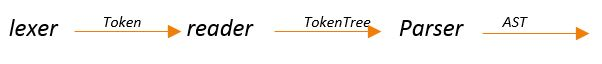
\includegraphics[width=0.5\textwidth]{images/Tokenizer.jpg}
\caption{Sweet.JS anatomy.} 
\label{fig:Tokenizer}
\end{figure}

Parser give structure to unstructured source code. lexer which converts a character stream to a token stream and a parser which converts the token stream into an AST according to a context free grammar ~\cite{bib2}.System which expand the macro definition must sit in between lexer and parser.Here reader records sufficiently history information in the form of token tree in order to decide how to parse the token, this is required to decide if token is a divisor or a regular expression.

Example

\begin{lstlisting}
		macro id {
  			case {_ $x } => {
   			 return #{ $x }
  			}
		  }
		id 42
\end{lstlisting}
Reader convert string of token to token tree, 
\begin{figure}[htb]
\centering
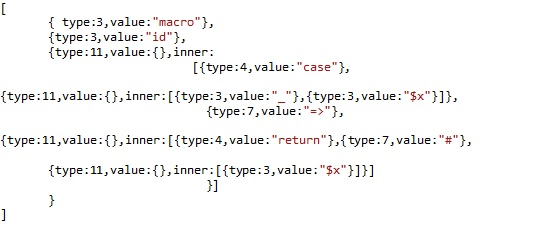
\includegraphics[width=1.0\textwidth]{images/readeroutput.jpg}
\caption{Token tree.} 
\label{fig:readeroutput}
\end{figure}

\begin{figure}[htb]
\centering
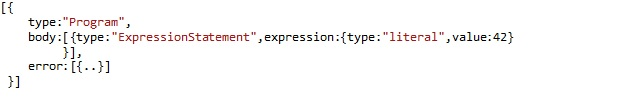
\includegraphics[width=1.0\textwidth]{images/AST.jpg}
\caption{Final AST from parser.} 
\label{fig:AST}
\end{figure}

The approach used in Sweet.JS named as Enforestation, was pioneered by Honu ~\cite{bib4}. Enforestation means transformation, it extract the sequence of terms produced by the reader to create a term tree. A term tree is a kind of proto-AST that represent the partial parse program. As the expander passes through the token trees, it creates term trees that contain unexpanded sub trees that will be expanded once all macro definition have been discovered in the current scope.



\section{Problem trying to solve?}

Although the benefits of hygienic macros are well established, there are occasions when traditional hygienic bindings are insufficient. let's understand this via example "anaphoric conditionals" where value of the tested expression is available as an 'it' bindings.That means when the condition is true, an "it" identifier is automatically created and set to the value of the condition.
\begin{figure}
\centering
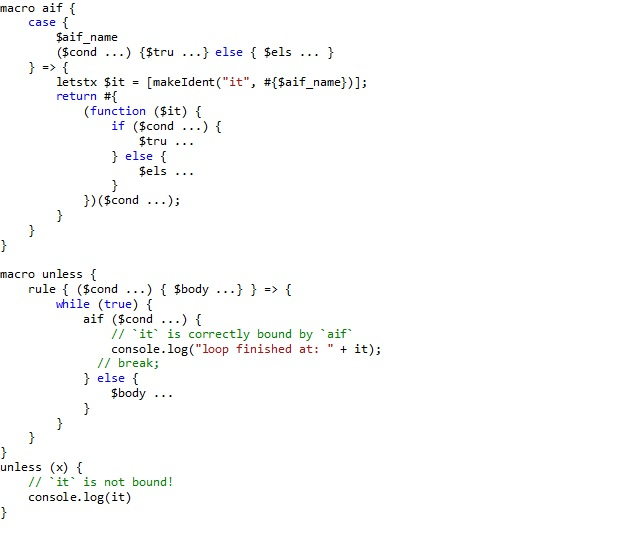
\includegraphics[width=1.0\textwidth]{images/Breakhygiene.jpg}
\caption{Break hygienic.} 
\label{fig:Breakhygiene}
\end{figure}

\begin{figure}
\centering
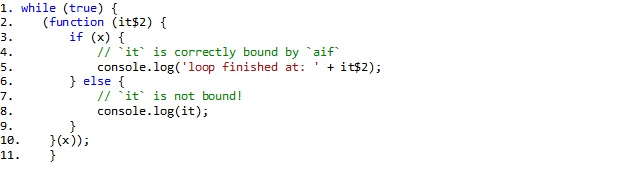
\includegraphics[width=1.0\textwidth]{images/macroexpansion.jpg}
\caption{Macro expansion.} 
\label{fig:macroexpansion}
\end{figure}

\newpage

In above macro expansion, at line (8) identifier 'it' is not defined.Here we wish to introduce the identifiers as is, unhygienically. Same unhygienic macros are observed in Scheme as shown in the below example, mistake is if our new syntax introduces a variable that accidentally conflicts with one in the code surrounding our macro.

\begin{lstlisting}
	(define-syntax-rule (aif condition true-expr false-expr)
    	(let ([it condition])
      	(if it
         	 true-expr
         	 false-expr)))

 	(aif #t (displayln it) (void))

	it: undefined;
	 cannot reference an identifier before its definition
  	in module: 'program
\end{lstlisting}

Good way is with a syntax parameter, as shown below inside the syntax-parameterize, "it" acts as an alias for tmp. The alias behavior is created by make-rename-transformer.\textbf{define-syntax-parameter}, binds keyword to the value obtained by evaluating transformer. The transformer provide the default expansion for the syntax parameter.
\textbf{syntax-parameterize}, adjust keyword to use the values obtained by evaluating their transformer in the expansion of the expression. 


\begin{lstlisting}
	(require racket/stxparam)
	(define-syntax-parameter it
    	(lambda (stx)
     	 (raise-syntax-error (syntax-e stx)
     	 		 "can only be used inside aif")))

 	(define-syntax-rule (aif condition true-expr false-expr)
    	(let ([tmp condition])
     	 (if tmp
          (syntax-parameterize ([it (make-rename-transformer #'tmp)])
            true-expr)
          false-expr)))
\end{lstlisting}

If we try to use it outside of an aif form, and it isn’t otherwise defined, we get an error 
\begin{lstlisting}
	(displayln it)

	error->it: can only be used inside aif
\end{lstlisting}

But we can still define it as a normal variable in local definition contexts like:
\begin{lstlisting}
	(let ([it 10])
  	  it)

	output: 10
\end{lstlisting}